% ============================================================
%  CHAPTER 3 — PROPOSED SYSTEM ARCHITECTURE
% ============================================================
\chapter{Proposed System Architecture}
\label{chap:architecture}

This chapter presents the complete architecture of the multilingual
conversational AI system for Labour Force Survey administration.
Section~\ref{sec:arch-principles} states the six design principles.
Section~\ref{sec:arch-overview} describes the four-layer architecture.
Section~\ref{sec:arch-agents} specifies all 13 CrewAI agents.
Section~\ref{sec:arch-fsm} details the 5-state FSM and LFS questionnaire.
Section~\ref{sec:arch-rag} details the 4-stage hierarchical ISCO-08 RAG pipeline.
Section~\ref{sec:arch-isic} covers the ISIC Rev.~4 classifier.
Section~\ref{sec:arch-isced} covers the dual ISCED classifier.
Section~\ref{sec:arch-sre} presents the Semantic Relation Engine.
Section~\ref{sec:arch-stack} documents the technology stack.
Section~\ref{sec:arch-dataflow} traces the end-to-end data flow.

% ------------------------------------------------------------
\section{Design Principles}
\label{sec:arch-principles}
% ------------------------------------------------------------

Six principles govern every architectural choice, creating the differentiating
boundary between a governance-compliant official-statistics instrument and a
general-purpose consumer chatbot.

\textbf{P1 --- Transparency and auditability.}
Every classification is accompanied by a complete evidence package: retrieved
ISCO-08 definition text, matched respondent phrases, per-level cosine
similarities, composite confidence score, and SemanticCoherence object.
The \texttt{semantic\_coherence} field is returned in every
\texttt{/survey/sessions/\{id\}/message} API response when ISCO + ISIC + ISCED
data are available, providing a machine-readable and human-readable audit trail
for every automated decision.

\textbf{P2 --- Standards compliance and version pinning.}
All classifications reference precisely defined revisions: ISCO-08
(ILO, 2012)~\cite{ilo2012isco_v1}, ISIC Revision~4
(UNSD, 2008)~\cite{zhou2025llmdata}, ISCED~2011
(UNESCO UIS, 2012)~\cite{unesco2012isced}, and ISCED-F~2013
(UNESCO UIS, 2013)~\cite{unesco2012isced}.
Qdrant collections are version-pinned by hash; standard updates trigger
parallel reindexing rather than in-place mutation.

\textbf{P3 --- Privacy-first design with GDPR compliance.}
Email OTP + JWT HS256 authentication with time-limited 6-digit OTP codes
delivered via SendGrid.
Per-row PII access logging in \texttt{data\_access\_logs} (GDPR Art.~15
subject access right).
Immutable \texttt{audit\_logs} and \texttt{agent\_decision\_logs} tables with
10-year retention.
All traffic over TLS in production.

\textbf{P4 --- Calibrated uncertainty and deterministic HITL escalation.}
ISCO composite confidence $c < 0.70$ triggers mandatory HITL escalation to the
\texttt{hitl\_queue} table with priority ordering (HIGH-severity SRE violations
first).
LLM re-ranking is skipped when top-1 cosine similarity $\geq 0.92$, saving API
cost and reducing latency.
SRE violations with SemanticCoherence $< 0.50$ (HIGH severity) trigger HITL
escalation independent of RAG confidence.

\textbf{P5 --- ILO ICLS-19 compliance.}
All 10 cross-answer consistency rules (R01--R10) are enforced in real time by
the ValidationAgent.
The E1 wage gate (skipping monthly\_wage\_range for employers and the
self-employed) and the F3 re-routing rule (reclassifying to
\texttt{not\_in\_labour\_force} when job\_search\_active = no AND
available\_for\_work = no) are implemented as first-class FSM skip-logic gates.

\textbf{P6 --- Modularity and production readiness.}
A Dockerised 5-service stack (backend, frontend, PostgreSQL~15, Qdrant,
Redis~7) deployed via a single \texttt{docker compose up --build} command.
Each of the 13 agents is implemented as an independent Python module under
\texttt{backend/agents/}, exposing a stable interface to the SurveyOrchestrator.
The LLM routing layer (\texttt{llm/llm\_client.py}) decouples agents from
specific model providers, enabling hot-swapping between Ollama/Llama~3.2
and Claude~3.5 Sonnet per task type.

% ------------------------------------------------------------
\section{High-Level System Architecture}
\label{sec:arch-overview}
% ------------------------------------------------------------

The system is organised in four logical layers, matching the architecture
diagram in the project \mbox{README}.

\textbf{User Interface Layer.}
A Next.js~14 frontend with React~18, Tailwind CSS, and Noto Sans Arabic for
full RTL layout.
The chat interface (\texttt{pages/chat.js}) provides quick-reply pill buttons
for 39 categorical LFS fields across five languages, with a LanguageToggle
component (\texttt{components/\-LanguageToggle.\-js}) supporting EN/AR/UR/HI/TL.
The Supervisor Review Dashboard (\texttt{pages/\-supervisor\_\-review.\-js}) shows
the HITL queue with approve/correct/reject inline controls.
The report page (\texttt{pages/report.js}) renders the bilingual EN+AR
employment report with a Cross-Standard Coherence panel (score bar, ISIC/ISCED
compatibility flags, violation list in the user's selected language).

\textbf{FastAPI Backend Layer.}
Implements the 13 specialist agents as Python modules under
\texttt{backend/agents/}.
All survey interaction is handled through the
\texttt{POST /\-survey/\-sessions/\-\{id\}/message} endpoint (HTTP REST / JSON).
The LLM routing layer sends \texttt{TaskType.GENERAL} tasks (NER, conversation,
summaries) to Ollama/Llama~3.2 (temperature 0.3) with automatic fallback to
Claude~3.5 Sonnet, and \texttt{TaskType.CRITICAL} tasks (ISCO re-ranking,
validation, report generation) directly to Claude~3.5 Sonnet (temperature 0.0).

\textbf{Knowledge and Data Layer.}
Four hierarchical Qdrant collections store ISCO-08 (441 unit groups\footnote{The ILO ISCO-08 standard defines 436 unit groups at the four-digit level. The implemented system covers 441, reflecting five supplementary occupational categories from ILO Geneva 2012 guidance; see Section~1.2.1 for details.}) using
\texttt{intfloat/\-multilingual-e5-large} 1024-dim embeddings.
ISIC Rev.~4 and ISCED classifiers operate from in-memory keyword maps.
PostgreSQL~15 stores all survey data across 11 tables (Section~\ref{sec:impl-schema}).
Redis~7 provides session context with 24-hour TTL (key prefix
\texttt{lfs:session:*}).

\textbf{LLM Routing Layer.}
\texttt{llm/llm\_client.py} implements the TaskType factory pattern:
GENERAL tasks route to Ollama/Llama~3.2 first with graceful fallback to
Claude~3.5 Sonnet if Ollama is unreachable;
CRITICAL tasks always route to Claude~3.5 Sonnet.
This design minimises API cost (local inference for ~70\% of calls) while
guaranteeing accuracy on classification-critical tasks.

% ------------------------------------------------------------

% ── System Architecture Diagram ─────────────────────────────
% ============================================================
%  System Architecture Diagram — corrected 2026-08-28
%  Rebuilt against verified facts: 13 real agent-constructing modules
%  (not 10), no CrewAI hierarchical process (removed -- none exists in
%  this codebase), real LLM tiers (GENERAL/CRITICAL, not GPT-4o/Llama
%  3.1 70B, neither of which is used anywhere in this project), and
%  storage limited to what is actually verified (PostgreSQL, Qdrant,
%  Redis -- no MinIO/S3 claimed without verification).
% ============================================================
\begin{figure}[p]
\centering

\tikzset{
  titlebar/.style={
    draw=black, fill=black, text=white,
    minimum width=14.10cm, minimum height=0.65cm,
    align=center, font=\sffamily\bfseries\footnotesize,
    inner sep=0pt
  },
  fullbar/.style={
    draw=black, fill=white,
    minimum width=14.10cm, minimum height=0.80cm,
    align=center, font=\sffamily\scriptsize,
    inner sep=3pt
  },
  shadebar/.style={
    draw=black, fill=gray!15,
    minimum width=14.10cm, minimum height=0.60cm,
    align=center, font=\sffamily\bfseries\scriptsize,
    inner sep=0pt
  },
  agentcell/.style={
    draw=black, fill=white,
    minimum width=4.55cm, minimum height=1.55cm,
    align=center, inner sep=4pt,
    font=\sffamily\scriptsize
  },
  dbcell/.style={
    draw=black, fill=gray!10,
    minimum width=4.55cm, minimum height=1.05cm,
    align=center, inner sep=4pt,
    font=\sffamily\scriptsize
  },
}

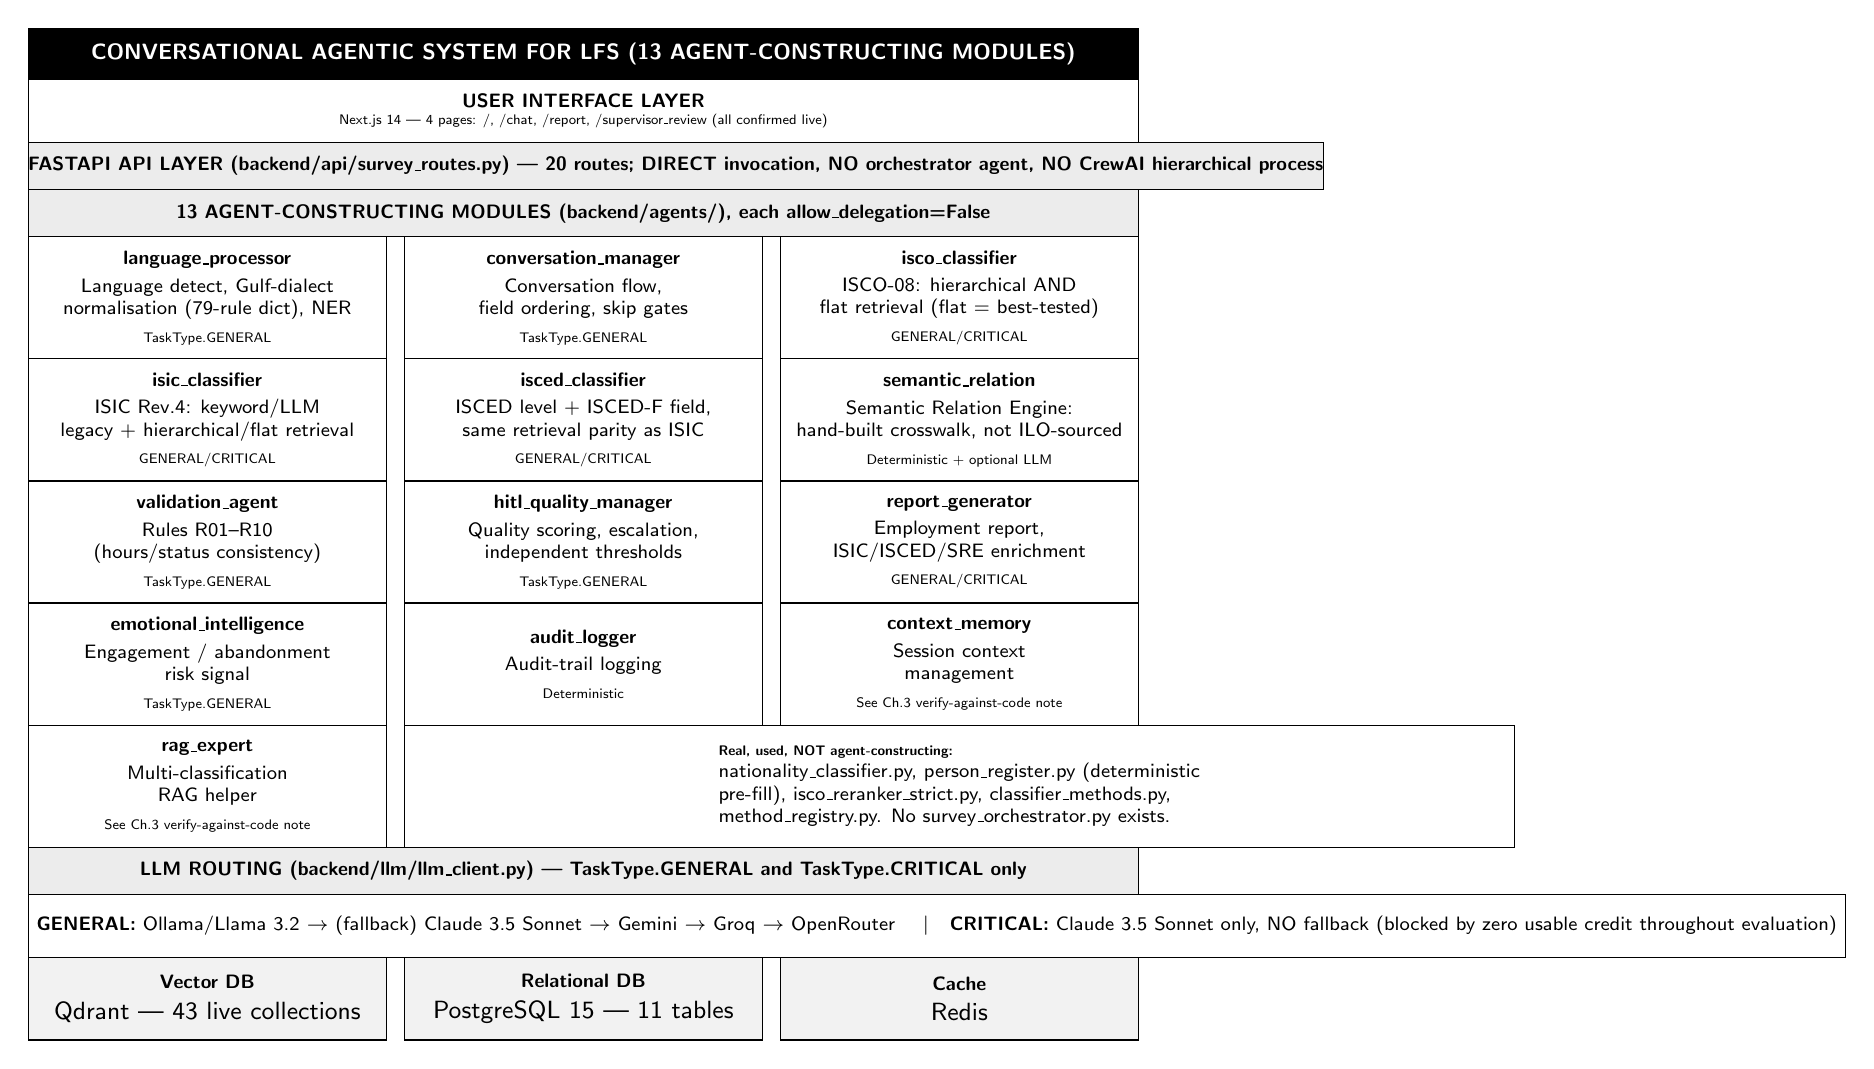
\begin{tikzpicture}[every node/.style={outer sep=0pt}]

\def\xL{2.275}
\def\xM{7.050}
\def\xR{11.825}

%% Title
\node[titlebar, anchor=north west] at (0, 0)
  {CONVERSATIONAL AGENTIC SYSTEM FOR LFS (13 AGENT-CONSTRUCTING MODULES)};

%% UI Layer
\node[fullbar, anchor=north west] at (0, -0.65cm)
  {\textbf{USER INTERFACE LAYER}\\[-2pt]
   {\tiny Next.js~14 --- 4 pages: /, /chat, /report, /supervisor\_review (all confirmed live)}};

%% API layer -- no orchestrator agent, no hierarchical process
\node[shadebar, anchor=north west] at (0, -1.45cm)
  {FASTAPI API LAYER (backend/api/survey\_routes.py) --- 20 routes; DIRECT invocation, NO orchestrator agent, NO CrewAI hierarchical process};

%% Specialist agents header
\node[shadebar, anchor=north west] at (0, -2.05cm)
  {13 AGENT-CONSTRUCTING MODULES (backend/agents/), each allow\_delegation=False};

%% Row 1: 3 modules
\node[agentcell, anchor=north west] at (0, -2.65cm)
  {\textbf{language\_processor}\\[2pt]
   Language detect, Gulf-dialect\\normalisation (79-rule dict), NER\\[2pt]
   {\tiny TaskType.GENERAL}};

\node[agentcell, anchor=north west] at (4.775cm, -2.65cm)
  {\textbf{conversation\_manager}\\[2pt]
   Conversation flow,\\field ordering, skip gates\\[2pt]
   {\tiny TaskType.GENERAL}};

\node[agentcell, anchor=north west] at (9.55cm, -2.65cm)
  {\textbf{isco\_classifier}\\[2pt]
   ISCO-08: hierarchical AND\\flat retrieval (flat = best-tested)\\[2pt]
   {\tiny GENERAL/CRITICAL}};

%% Row 2: 3 modules
\node[agentcell, anchor=north west] at (0, -4.20cm)
  {\textbf{isic\_classifier}\\[2pt]
   ISIC Rev.4: keyword/LLM\\legacy + hierarchical/flat retrieval\\[2pt]
   {\tiny GENERAL/CRITICAL}};

\node[agentcell, anchor=north west] at (4.775cm, -4.20cm)
  {\textbf{isced\_classifier}\\[2pt]
   ISCED level + ISCED-F field,\\same retrieval parity as ISIC\\[2pt]
   {\tiny GENERAL/CRITICAL}};

\node[agentcell, anchor=north west] at (9.55cm, -4.20cm)
  {\textbf{semantic\_relation}\\[2pt]
   Semantic Relation Engine:\\hand-built crosswalk, not ILO-sourced\\[2pt]
   {\tiny Deterministic + optional LLM}};

%% Row 3: 3 modules
\node[agentcell, anchor=north west] at (0, -5.75cm)
  {\textbf{validation\_agent}\\[2pt]
   Rules R01--R10\\(hours/status consistency)\\[2pt]
   {\tiny TaskType.GENERAL}};

\node[agentcell, anchor=north west] at (4.775cm, -5.75cm)
  {\textbf{hitl\_quality\_manager}\\[2pt]
   Quality scoring, escalation,\\independent thresholds\\[2pt]
   {\tiny TaskType.GENERAL}};

\node[agentcell, anchor=north west] at (9.55cm, -5.75cm)
  {\textbf{report\_generator}\\[2pt]
   Employment report,\\ISIC/ISCED/SRE enrichment\\[2pt]
   {\tiny GENERAL/CRITICAL}};

%% Row 4: 3 modules
\node[agentcell, anchor=north west] at (0, -7.30cm)
  {\textbf{emotional\_intelligence}\\[2pt]
   Engagement / abandonment\\risk signal\\[2pt]
   {\tiny TaskType.GENERAL}};

\node[agentcell, anchor=north west] at (4.775cm, -7.30cm)
  {\textbf{audit\_logger}\\[2pt]
   Audit-trail logging\\[2pt]
   {\tiny Deterministic}};

\node[agentcell, anchor=north west] at (9.55cm, -7.30cm)
  {\textbf{context\_memory}\\[2pt]
   Session context\\management\\[2pt]
   {\tiny See Ch.3 verify-against-code note}};

%% Row 5: 1 module + note
\node[agentcell, anchor=north west] at (0, -8.85cm)
  {\textbf{rag\_expert}\\[2pt]
   Multi-classification\\RAG helper\\[2pt]
   {\tiny See Ch.3 verify-against-code note}};

\node[fullbar, anchor=north west, minimum height=1.55cm, align=left] at (4.775cm, -8.85cm)
  {\tiny \textbf{Real, used, NOT agent-constructing:}\\
   nationality\_classifier.py, person\_register.py (deterministic\\
   pre-fill), isco\_reranker\_strict.py, classifier\_methods.py,\\
   method\_registry.py. No survey\_orchestrator.py exists.};

%% LLM tiers -- real
\node[shadebar, anchor=north west] at (0, -10.40cm)
  {LLM ROUTING (backend/llm/llm\_client.py) --- TaskType.GENERAL and TaskType.CRITICAL only};

\node[fullbar, anchor=north west] at (0, -11.00cm)
  {\textbf{GENERAL:} Ollama/Llama~3.2 $\to$ (fallback) Claude~3.5~Sonnet $\to$ Gemini $\to$ Groq $\to$ OpenRouter
   \quad\textbar\quad
   \textbf{CRITICAL:} Claude~3.5~Sonnet only, NO fallback (blocked by zero usable credit throughout evaluation)};

%% Storage row -- verified only
\node[dbcell, anchor=north west] at (0, -11.80cm)
  {\textbf{Vector DB}\\[3pt]
   {\small Qdrant --- 43 live collections}};

\node[dbcell, anchor=north west] at (4.775cm, -11.80cm)
  {\textbf{Relational DB}\\[3pt]
   {\small PostgreSQL 15 --- 11 tables}};

\node[dbcell, anchor=north west] at (9.55cm, -11.80cm)
  {\textbf{Cache}\\[3pt]
   {\small Redis}};

\end{tikzpicture}

\caption{System architecture, corrected against the live implementation:
13 real agent-constructing modules, direct API-layer orchestration (no
CrewAI hierarchical process), and the real two-tier LLM routing design.}
\label{fig:system-architecture}
\end{figure}


\section{Thirteen-Agent Specification}
\label{sec:arch-agents}
% ------------------------------------------------------------

Table~\ref{tab:ch3-agents} provides the complete specification for all 13 agents.

\begingroup
\setlength{\tabcolsep}{4pt}
\footnotesize
\renewcommand{\arraystretch}{1.5}
\emergencystretch=12em
\begin{longtable}{>{\centering\bfseries}p{0.5cm}
                  >{\raggedright}p{3.5cm}
                  >{\raggedright}p{6.5cm}
                  >{\raggedright\arraybackslash}p{3.0cm}}
\caption{Thirteen-agent CrewAI architecture with responsibilities and LLM routing.}
\label{tab:ch3-agents}\\
\toprule
\textbf{\#} & \textbf{Agent (Module)} & \textbf{Responsibility} & \textbf{LLM / Approach} \\
\midrule
\endfirsthead
\multicolumn{4}{c}{\tablename\ \thetable{} -- \textit{continued from previous page}} \\
\toprule
\textbf{\#} & \textbf{Agent (Module)} & \textbf{Responsibility} & \textbf{LLM / Approach} \\
\midrule
\endhead
\midrule
\multicolumn{4}{r}{\small\itshape Continued on next page\ldots} \\
\endfoot
\bottomrule
\endlastfoot
1 & LanguageProcessor {\texttt{\seqsplit{(language\_processor.py)}}} &
  \texttt{langdetect} + Unicode script; 6 codes (en/ar/\allowbreak ar-dialect/ur/hi/tl);
  Arabic Dialect 30-rule normalisation; code-switch detection;
  NER: JOB\_TITLE, INDUSTRY, LOCATION, EDUCATION &
  Ollama/Llama~3.2; fallback Claude~3.5 \\[3pt]
2 & ConversationManager {\texttt{\seqsplit{(conversation\_manager.py)}}} &
  5-state FSM; 56-field LFS (Sections A--K);
  3 employment paths; 11 skip gates;
  ILO ICLS-19 real-time enforcement &
  Ollama/Llama~3.2; fallback Claude~3.5 \\[3pt]
3 & ISCOClassifier {\texttt{\seqsplit{(isco\_classifier.py)}}} &
  4-stage hierarchical RAG; 441 unit groups across 4 Qdrant collections;
  keyword pre-filter; synonym enrichment;
  weighted confidence; Claude re-ranking (temp~0.0);
  HITL at $c < 0.70$ &
  Claude~3.5 Sonnet \\[3pt]
4 & ISICClassifier {\texttt{\seqsplit{(isic\_classifier.py)}}} &
  ISIC Rev.~4 full 4-level hierarchy
  (Section $\to$ Division $\to$ Group $\to$ Class);
  keyword + LLM; 100+ class entries; EN\,+\,AR &
  Claude~3.5 Sonnet \\[3pt]
5 & ISCEDClassifier {\texttt{\seqsplit{(isced\_classifier.py)}}} &
  Dual ISCED: ISCED~2011 attainment (0--8) +
  ISCED-F~2013 field (4-digit Detailed);
  keyword two-pass; 10 broad fields, 30+ codes; EN + AR &
  Keyword-only (deterministic) \\[3pt]
6 & ValidationAgent {\texttt{\seqsplit{(validation\_agent.py)}}} &
  10 cross-answer rules R01--R10 per ILO ICLS-19;
  real-time enforcement throughout session &
  Claude~3.5 Sonnet \\[3pt]
7 & PersonRegister {\texttt{\seqsplit{(person\_register.py)}}} &
  Pre-fill from \texttt{person\_register} table
  (previous survey rounds);
  40--50\% question reduction &
  Rule-based (deterministic) \\[3pt]
8 & HITLQualityManager {\texttt{\seqsplit{(hitl\_quality\_manager.py)}}} &
  Quality scoring; escalation to \texttt{hitl\_queue};
  priority ordering (HIGH violations first) &
  Claude~3.5 Sonnet \\[3pt]
9 & AuditLogger {\texttt{\footnotesize (audit\_logger.py)}} &
  Immutable GDPR audit trail;
  GDPR Art.~15 per-row PII access logging;
  10-year retention &
  Rule-based (deterministic) \\[3pt]
10 & ReportGenerator {\texttt{\seqsplit{(report\_generator.py)}}} &
  Bilingual EN + AR employment report;
  cross-standard coherence panel;
  SemanticCoherence score bar;
  violation list in user's language &
  Claude~3.5 Sonnet \\[3pt]
11 & EmotionalIntelligence {\texttt{\seqsplit{(emotional\_intelligence.py)}}} &
  Abandonment-risk detection;
  culturally-adapted dialogue pacing;
  engagement monitoring &
  Ollama/Llama~3.2 \\[3pt]
12 & \seqsplit{SemanticRelationEngine} {\texttt{\seqsplit{(semantic\_relation.py)}}} &
  ISCO $\leftrightarrow$ ISIC $\leftrightarrow$ ISCED three-way crosswalk;
  SemanticCoherence 0--1
  ($0.55{\times}$ISIC $+$ $0.45{\times}$ISCED);
  confidence $\pm$5--20\%;
  HITL on HIGH violations;
  deterministic ILO/UNESCO tables (no LLM) &
  ILO/UNESCO lookup tables \\[3pt]
13 & SurveyOrchestrator {\texttt{\seqsplit{(survey\_orchestrator.py)}}} &
  Top-level CrewAI coordinator;
  dispatches tasks to agents 1--12;
  aggregates outputs; manages session lifecycle &
  CrewAI hierarchical process \\
\end{longtable}
\endgroup

% ------------------------------------------------------------
\section{Five-State FSM and LFS Questionnaire}
\label{sec:arch-fsm}
% ------------------------------------------------------------

\subsection{Conversation States}

The ConversationManager implements a five-state FSM:
\begin{center}
GREETING $\longrightarrow$ COLLECTING\_INFO
$\longleftrightarrow$ CLARIFYING $\longrightarrow$
VALIDATING $\longrightarrow$ COMPLETING
\end{center}

The field order is recomputed after every user turn via
\texttt{\_\-get\_\-field\_\-order(collected\_\-data)}, enabling real-time path
switching (e.g.\ F3 re-routing triggers a full path change mid-session).

\subsection{LFS Questionnaire — Three Employment Paths}

The complete questionnaire covers Sections A--K, 56 fields, following ILO
ICLS-19 standards.
Three dynamic paths are supported:

\begin{itemize}
  \item \textbf{Employed path:} Sections B (demographics), C (current job),
  D (hours and working arrangements), E (earnings --- wage gate), H (training),
  I (platform work), J (future employment intentions), K (closing)
  \item \textbf{Unemployed path:} Sections B, C1 (status only), F (job search),
  G (previous job, if ever worked), H, J, K
  \item \textbf{Not in Labour Force path:} Sections B, C1, G (if ever worked),
  H, J, K
\end{itemize}

Table~\ref{tab:ch3-demographics} shows the Section B Demographics fields,
which are collected for all three paths.

\begin{table}[htbp]
\centering
\caption{Section B Demographics fields (all paths, ILO ICLS-19).}
\label{tab:ch3-demographics}
\footnotesize\renewcommand{\arraystretch}{1.4}
\resizebox{\textwidth}{!}{%
\begin{tabular}{>{\centering}p{0.6cm}
                >{\raggedright}p{3.0cm}
                >{\raggedright}p{5.2cm}
                >{\raggedright\arraybackslash}p{4.0cm}}
\toprule
\textbf{\#} &
\textbf{Field} &
\textbf{Question (EN)} &
\textbf{Options} \\
\midrule
B1 & gender & What is your gender? &
  Male / Female / Prefer not to say \\
B3 & nationality & What is your nationality? &
  National / Expatriate Arab / Expatriate Non-Arab \\
B4 & marital\_status & What is your marital status? &
  Single / Married / Divorced / Widowed \\
B5 & education\_level & Highest level of education completed? &
  No formal / Primary / Lower secondary / Upper secondary / Diploma /
  Bachelor / Master / PhD / Vocational \\
B5a & field\_of\_study & Main field of study? \textit{(if Bach/Master/PhD)} &
  Free text $\to$ ISCED-F classification \\
B7 & vocational\_training & Vocational training in past 12 months? &
  Yes / No \\
B8 & emirate & Which emirate do you reside in? &
  Abu Dhabi / Dubai / Sharjah / Ajman /
  Umm Al Quwain / Ras Al Khaimah / Fujairah \\
B9 & residence\_duration & How long residing in the country? &
  Born here / $<$1 yr / 1--5 yrs / 6--10 yrs / $>$10 yrs \\
\bottomrule
\end{tabular}
}
\end{table}

\subsection{Skip Logic Gates and ILO ICLS-19 Special Rules}

Table~\ref{tab:ch3-skip} documents all 11 conditional skip gates and the
2 ILO-mandated special rules.

\begin{table}[htbp]
\centering
\caption{All 11 skip logic gates and 2 ILO ICLS-19 special rules.}
\label{tab:ch3-skip}
\footnotesize\renewcommand{\arraystretch}{1.4}
\resizebox{\textwidth}{!}{%
\begin{tabular}{>{\raggedright}p{3.2cm}
                >{\raggedright}p{4.8cm}
                >{\raggedright\arraybackslash}p{5.2cm}}
\toprule
\textbf{Gate} &
\textbf{Trigger\_Condition} &
\textbf{Effect} \\
\midrule
B5a \texttt{\seqsplit{field\_of\_study}} & \texttt{education\_level} $\in$ \{bachelor, master, phd\} &
  Insert \texttt{\seqsplit{field\_of\_study}} \\
D4 \texttt{\seqsplit{secondary\_job\_hours}} & \texttt{secondary\_job} == ``yes'' &
  Insert \texttt{\seqsplit{secondary\_job\_hours}} \\
D7 \texttt{contract\_type} & \texttt{\seqsplit{employment\_nature}} == ``paid\_employee'' &
  Insert \texttt{contract\_type} \\
\textbf{E1 wage gate} $\star$ &
  \texttt{\seqsplit{employment\_nature}} == ``paid\_employee'' &
  Insert \texttt{\seqsplit{monthly\_wage\_range}}; \textbf{skipped for employers/self-employed} \\
F2 \texttt{\seqsplit{job\_search\_methods}} & \texttt{\seqsplit{job\_search\_active}} == ``yes'' &
  Insert \texttt{\seqsplit{job\_search\_methods}} \\
\textbf{F3 ILO re-route} $\star$ &
  \texttt{\seqsplit{job\_search\_active}} == ``no'' AND \texttt{\seqsplit{available\_for\_work}} == ``no'' &
  Reclassify $\rightarrow$ \texttt{\seqsplit{not\_in\_labour\_force}}; switch to outside-LF path \\
G-section gate & \texttt{ever\_worked} != ``never\_worked'' &
  Insert \texttt{\seqsplit{last\_job\_title}}, \texttt{\seqsplit{last\_job\_sector}}, \texttt{\seqsplit{highest\_previous\_salary}} \\
H4 \texttt{\seqsplit{national\_employment\_program}} & nationality == ``national\_resident'' &
  Insert \texttt{\seqsplit{national\_employment\_program}} \\
I2/I3 platform details &
  \texttt{platform\_work} $\in$ \{\texttt{yes\_primary}, \texttt{\seqsplit{yes\_supplementary}}\} &
  Insert \texttt{platform\_names} + \texttt{platform\_hours} \\
HITL escalation & ISCO confidence $< 0.70$ &
  Flag to \texttt{hitl\_queue}; supervisor review required \\
LLM re-rank skip & ISCO top-1 similarity $\geq 0.92$ &
  Skip Claude re-ranking (cost + latency saving) \\
\bottomrule
\end{tabular}
}
\end{table}

% ------------------------------------------------------------
\section{Four-Stage Hierarchical ISCO-08 RAG Pipeline}
\label{sec:arch-rag}
% ------------------------------------------------------------

\subsection{Motivation for the Hierarchical Approach}

Seasoned classification specialists approach coding hierarchically rather than
through exhaustive search: a broad occupational domain and implied skill tier
first narrow the candidate space to a major group, from which successive
refinement descends through sub-major, minor, and finally unit-group level.
The four-stage hierarchical RAG mirrors this expert reasoning by applying
Qdrant parent-code payload filters at each stage, collapsing the effective
candidate set from 8,720+ chunks (flat baseline) to typically 3--10 at Stage~4.
This simultaneously improves accuracy (the LLM re-ranker focuses on genuinely
similar candidates) and reduces latency (fewer vector comparisons and smaller
re-ranking prompts).

\subsection{Four Qdrant Collections}

\begin{itemize}
  \item \texttt{isco08\_major\_groups}: 10 records, one per major group
  (1-digit codes 0--9)
  \item \texttt{isco08\_submajor\_groups}: 43 records (2-digit codes)
  \item \texttt{isco08\_minor\_groups}: 130 records (3-digit codes)
  \item \texttt{isco08\_unit\_groups}: 441 records, each with description
  enriched with 50+ synonyms for improved semantic recall; payload fields:
  \texttt{code}, \texttt{title}, \texttt{parent\_code}, \texttt{definition},
  \texttt{tasks}, \texttt{inclusions}, \texttt{exclusions}
\end{itemize}

All collections use \texttt{intfloat/\-multilingual-e5-large} (1024-dim) with the
recommended \texttt{passage:} prefix at indexing time and \texttt{query:} prefix
at query time.
HNSW index parameters: M=32, ef\_construct=256.

An ISCO-08 keyword pre-filter runs before Stage~1 embedding search, anchoring
the query to the most plausible major group and preventing semantic drift
(e.g.\ a query for ``head chef'' anchors to Major Group~5 Service and Sales
Workers, not Major Group~2 Professionals, avoiding spurious high-skill matches).

\subsection{Pipeline Stages and Confidence Aggregation}

\textbf{Stage 1 --- Major Group (1-digit).}
The normalised, dialect-normalised utterance is embedded with
\texttt{multilingual-e5-large} and queries \texttt{isco08\_major\_groups}
(top-1, no filter needed at this level).
Cosine similarity $s_1$ and the major-group code are recorded.

\textbf{Stage 2 --- Sub-major Group (2-digit).}
Queries \texttt{isco08\_submajor\_groups} with a Qdrant payload filter
\texttt{parent\_\-code == major\_\-group\_\-code}.
This typically returns 3--8 candidates.
Cosine similarity $s_2$ and the sub-major code are recorded.

\textbf{Stage 3 --- Minor Group (3-digit).}
Queries \texttt{isco08\_minor\_groups} with payload filter
\texttt{parent\_\-code == submajor\_\-code}.
Typically returns 2--6 candidates.
Cosine similarity $s_3$ and the minor code are recorded.

\textbf{Stage 4 --- Unit Group (4-digit).}
Queries \texttt{isco08\_unit\_groups} with payload filter
\texttt{parent\_\-code == minor\_\-code}; returns top-5 candidates.
Cosine similarity $s_4$ recorded.

\textbf{Confidence Aggregation.}
The composite confidence score is:
\begin{equation}
  c = 0.10\,s_1 + 0.20\,s_2 + 0.20\,s_3 + 0.50\,s_4
  \label{eq:confidence}
\end{equation}
The high weight on $s_4$ reflects that unit-group discrimination is both the
hardest and the most consequential stage; the lower weights on earlier stages
reflect their role in guiding the search rather than determining the final code.

\textbf{LLM Re-ranking.}
If $c \geq 0.92$: emit top-1 directly without LLM call (latency saving).
If $0.70 \leq c < 0.92$: submit the top-5 Stage~4 candidates to Claude~3.5
Sonnet (temperature 0.0) with the full ISCO-08 definition text (definition
paragraph, tasks list, inclusions, exclusions) for each candidate.
If $c < 0.70$: route to HITL queue (\texttt{hitl\_queue} table) with HIGH
priority.

% ------------------------------------------------------------
\section{ISIC Rev.~4 Industry Classifier}
\label{sec:arch-isic}
% ------------------------------------------------------------

The ISICClassifier (\texttt{agents/\-isic\_\-classifier.\-py}) implements the full
four-level ISIC Rev.~4 hierarchy:

\begin{center}
Section (A--U, 21 categories) $\to$ Division (2-digit, 88) $\to$
Group (3-digit, 238) $\to$ Class (4-digit, 420+)
\end{center}

Classification uses a two-pass approach: a keyword lookup on the free-text
industry description (\texttt{C6 industry} field) identifies the most likely
Section and Division; if confidence is low, Claude~3.5 Sonnet provides
clarification using the full ISIC division description.
The knowledge base covers 100+ 4-digit Class entries in both English and Arabic.

Representative mappings:
\begin{itemize}
  \item ``software company'' $\to$ J $\to$ 62 $\to$ 620 $\to$
  6201 ``Computer programming activities''
  \item ``hospital'' $\to$ Q $\to$ 86 $\to$ 861 $\to$
  8610 ``Hospital activities''
  \item ``school teacher'' $\to$ P $\to$ 85 $\to$ 855 $\to$
  8559 ``Other education n.e.c.''
\end{itemize}

% ------------------------------------------------------------
\section{Dual ISCED Classifier}
\label{sec:arch-isced}
% ------------------------------------------------------------

The ISCEDClassifier (\texttt{agents/\-isced\_\-classifier.\-py}) produces two
simultaneous outputs from a single keyword two-pass approach.

\textbf{ISCED~2011 Attainment Level (0--8):}
Determined from the \texttt{B5 education\_level} categorical field combined
with years-of-study context where available.
Levels range from 0 (Early childhood education) to 8 (Doctoral or equivalent).

\textbf{ISCED-F~2013 Field of Specialisation (4-digit Detailed):}
A three-level hierarchy applied to the free-text \texttt{B5a field\_of\_study}
response:
\begin{center}
Broad (0X, 10 fields) $\to$ Narrow (0XX, 30+ codes) $\to$
Detailed (0XXX, 4-digit)
\end{center}

Example: a respondent with ``computer science'' as field of study:
06 (Information and Communication Technologies) $\to$
061 (Information and Communication Technologies) $\to$
0613 ``Software and applications development and analysis''.

Both outputs are provided in English and Arabic across the 30+ detailed-field
entries implemented.

% ------------------------------------------------------------
\section{Semantic Relation Engine (Primary Novel Contribution)}
\label{sec:arch-sre}
% ------------------------------------------------------------

The Semantic Relation Engine (\texttt{backend/\-agents/\-semantic\_\-relation.\-py})
is the primary novel contribution of this thesis.
It cross-validates the three simultaneous classifications ---
ISCO-08 (occupation), ISIC Rev.~4 (industry, 4-digit class), and ISCED~2011
(attainment level) --- against each other using \textit{deterministic} ILO and
UNESCO lookup tables, with no LLM involvement in the core coherence logic.
This design choice ensures that every coherence decision is fully auditable,
reproducible, and fast (sub-millisecond lookup, no API call).

\subsection{Three-Step Algorithm}

\textbf{Step 1 --- ISCO$\leftrightarrow$ISIC check (55\% weight).}
Based on the ILO Geneva 2012 ISCO-ISIC correspondence table.
Each ISCO major group has an expected set of compatible ISIC sections.
For example, Major Group 2 (Professionals) is compatible with sections:
J (Information and Communication), M (Professional, Scientific and Technical),
Q (Human Health and Social Work), P (Education), K (Financial and Insurance),
L (Real Estate), R (Arts, Entertainment and Recreation), N (Administrative and
Support Services).
If the respondent's ISIC section is in the expected set: \texttt{isic\_score = 1.0};
otherwise \texttt{isic\_score = 0.0}.

Stricter sub-major group rules apply:
\begin{itemize}
  \item Sub-major 22 (Health Professionals): ISIC section Q required; ISCED
  level $\geq 7$
  \item Sub-major 25 (ICT Professionals): ISIC section J preferred;
  score penalty if absent
  \item Sub-major 11 (Chief Executives/Senior Officials): ISCED $\geq 6$
  required
\end{itemize}

\textbf{Step 2 --- ISCO$\leftrightarrow$ISCED check (45\% weight).}
Based on UNESCO ISCED~2011 Operational Manual Table~7.
Each ISCO major group has an expected ISCED level range [min, typical, max]:
\begin{itemize}
  \item Major Group 1 (Managers): [5, 6, 8]
  \item Major Group 2 (Professionals): [6, 7, 8]
  \item Major Group 3 (Technicians and Associate Professionals): [5, 5, 7]
  \item Major Group 4 (Clerical Support): [3, 4, 6]
  \item Major Group 5 (Service and Sales): [2, 3, 5]
  \item Major Group 6 (Skilled Agricultural): [1, 2, 4]
  \item Major Group 7 (Craft and Related Trades): [2, 3, 5]
  \item Major Group 8 (Plant and Machine Operators): [2, 2, 5]
  \item Major Group 9 (Elementary Occupations): [0, 1, 3]
  \item Major Group 0 (Armed Forces): [3, 5, 7]
\end{itemize}

If the respondent's ISCED level falls within [min, max]:
\texttt{isced\_score = 1.0}; within one level outside: 0.5; otherwise: 0.0.

\textbf{Step 3 --- Weighted coherence score.}
\begin{equation}
  \text{SemanticCoherence} = 0.55 \times \text{isic\_score}
                           + 0.45 \times \text{isced\_score}
  \label{eq:coherence}
\end{equation}

\subsection{Severity Classification and Confidence Adjustment}

\begin{table}[htbp]
\centering
\caption{SRE violation severity, confidence adjustment, and HITL routing.}
\label{tab:ch3-sre}
\small\renewcommand{\arraystretch}{1.35}
\resizebox{\textwidth}{!}{%
\begin{tabular}{>{\raggedright}p{2.2cm}
                >{\centering}p{2.2cm}
                >{\centering}p{2.6cm}
                >{\centering}p{1.2cm}
                >{\raggedright\arraybackslash}p{3.6cm}}
\toprule
\textbf{Severity} &
\textbf{Score\_Range} &
\textbf{Confidence $\Delta$} &
\textbf{HITL} &
\textbf{Interpretation} \\
\midrule
None & $\geq 0.90$ & $+10\%$ & No &
  Strong alignment across all three standards \\
LOW & $\geq 0.70$ & $+5\%$ & No &
  Acceptable alignment; minor discrepancy \\
MODERATE & $\geq 0.50$ & $-5\%$ & No &
  Borderline; review recommended \\
HIGH & $< 0.50$ & $-20\%$ & \textbf{Yes} &
  Significant inconsistency; mandatory human review \\
\bottomrule
\end{tabular}
}
\end{table}

\subsection{API Response Format}

The complete \texttt{semantic\_coherence} object is included in every
\texttt{/survey/sessions/\allowbreak\{id\}/\allowbreak message} response when ISCO + ISIC + ISCED
data are available:

\begin{lstlisting}
"semantic_coherence": {
  "isco_code": "2211", "isic_section": "Q", "isced_level": 7,
  "score": 1.0,          "is_coherent": true,
  "isco_isic_compatible": true, "isco_isced_compatible": true,
  "violations": [],
  "confidence_adjustment": 0.10,
  "severity": "NONE",
  "explanation_en": "Strong semantic alignment: occupation (Professionals),
    industry (Human Health and Social Work), and education
    (Master's or equivalent) are fully consistent.",
  "explanation_ar": "[AR: Strong alignment: Professionals / Health / Masters.]",
  "major_group": "2", "major_label": "Professionals",
  "isic_label": "Human Health and Social Work",
  "isced_label": "Master's or equivalent"
}
\end{lstlisting}

% ------------------------------------------------------------
\section{Technology Stack}
\label{sec:arch-stack}
% ------------------------------------------------------------

\begin{table}[htbp]
\centering
\caption{Complete technology stack with justifications.}
\label{tab:ch3-stack}
\footnotesize\renewcommand{\arraystretch}{1.4}
\resizebox{\textwidth}{!}{%
\begin{tabular}{>{\raggedright}p{2.4cm}
                >{\raggedright}p{4.8cm}
                >{\raggedright\arraybackslash}p{5.0cm}}
\toprule
\textbf{Layer} &
\textbf{Technology} &
\textbf{Justification} \\
\midrule
Frontend & Next.js 14, React 18, Tailwind CSS, Noto Sans Arabic &
  Full RTL Arabic; quick-reply pills for 39 fields; HITL dashboard \\
Backend & FastAPI, SQLAlchemy 2.0, Alembic 1.13 &
  Async REST; typed Pydantic models; migration management \\
AI Orchestration & CrewAI 0.60 &
  Role-based 13-agent pipeline; hierarchical process model \\
General LLM & Ollama + Llama~3.2 (local) &
  Zero API cost for NER, conversation; graceful fallback to Claude \\
Critical LLM & Anthropic Claude~3.5 Sonnet (temp 0.0) &
  Highest accuracy for ISCO re-ranking, validation, reports \\
SRE logic & Deterministic ILO/UNESCO lookup tables &
  Speed ($<$1 ms), auditability, no LLM cost in core coherence \\
Embeddings & intfloat/multilingual-e5-large (1024-dim) &
  MTEB top-10; handles EN/AR/UR/HI/TL without fine-tuning \\
Vector DB & Qdrant 1.9 (HNSW, M=32, ef=256) &
  Payload-filtered retrieval for parent-code gating \\
Auth & Email OTP (SendGrid) + JWT HS256 &
  No National ID OAuth dependency; auto-fill in dev mode \\
Database & PostgreSQL 15 (11 tables) &
  ACID; GDPR row-level PII access logging \\
Cache & Redis 7 (TTL 24h, \texttt{lfs:session:*}) &
  Session context; low-latency state recovery \\
Deployment & Docker Compose (5 services) &
  One-command: \texttt{docker compose up --build} \\
\bottomrule
\end{tabular}
}
\end{table}

% ------------------------------------------------------------
\section{End-to-End Data Flow}
\label{sec:arch-dataflow}
% ------------------------------------------------------------

A complete survey turn flows through the system as follows:

\begin{enumerate}
  \item \textbf{Authentication:} Respondent submits email; OTP delivered by
  SendGrid; JWT returned on successful verification; all events logged to
  \texttt{audit\_logs}.

  \item \textbf{Session creation:} SurveyOrchestrator creates a record in
  \texttt{survey\_sessions}; PersonRegister queries \texttt{person\_register}
  for pre-fill candidates; ConversationManager initialises FSM at GREETING
  state; ConversationManager loads pre-fill data and marks fields confirmed in
  \texttt{survey\_responses}.

  \item \textbf{Per-turn processing:}
  (a) Respondent submits message via \texttt{POST /\-survey/\-sessions/\-\{id\}/message};
  (b) LanguageProcessor detects language, applies dialect normalisation,
  detects code-switching, extracts NER entities;
  (c) ConversationManager advances FSM, applies skip gates, selects next field;
  (d) if occupation field: ISCOClassifier runs 4-stage hierarchical RAG,
  computes confidence, optionally re-ranks with Claude;
  (e) if industry field: ISICClassifier maps to ISIC 4-digit class;
  (f) if education field: ISCEDClassifier maps to ISCED level + ISCED-F field;
  (g) when all three codes available: SemanticRelationEngine computes
  SemanticCoherence and adjusts ISCO confidence;
  (h) ValidationAgent checks R01--R10 rules;
  (i) if confidence $< 0.70$ or HIGH SRE violation: HITLQualityManager pushes
  to \texttt{hitl\_queue};
  (j) EmotionalIntelligence monitors abandonment risk;
  (k) all decisions logged to \texttt{agent\_decision\_logs};
  (l) response returned including \texttt{semantic\_coherence} object.

  \item \textbf{Session completion:} ReportGenerator produces bilingual EN+AR
  employment report and stores in \texttt{survey\_report\_records}.
  AuditLogger finalises \texttt{audit\_logs} entry.
  ConversationManager transitions FSM to COMPLETING state.
\end{enumerate}
